\documentclass[11pt, oneside]{article} 	% use "amsart" instead of "article" for AMSLaTeX format
\usepackage{geometry} 		% See geometry.pdf to learn the layout options. There are lots.
\geometry{letterpaper}  		% ... or a4paper or a5paper or ... 
\usepackage[parfill]{parskip} 		% Activate to begin paragraphs with an empty line rather than an indent
\usepackage{graphicx}				% Use pdf, png, jpg, or eps§ with pdflatex; use eps in DVI mode
								% TeX will automatically convert eps --> pdf in pdflatex		
\usepackage{amssymb}
\usepackage{amsmath}
\usepackage{authblk}
\usepackage[
backend=biber,
style=alphabetic,
]{biblatex}
\usepackage{graphicx}
\graphicspath{ {./images/} }
\usepackage{verbatim}
\usepackage{tikz} 
\tikzset{
    vertex/.style={circle,draw,minimum size=1.5em},
    edge/.style={->,> = latex'}
}
\usetikzlibrary{arrows}
\usepackage{subcaption}
\usepackage{hyperref}
\usepackage{xcolor,colortbl}

\usepackage{listings}
\lstset{
basicstyle=\small\ttfamily,
columns=flexible,
breaklines=true
}
\usepackage{syntonly}
% \syntaxonly <-- use this for checking syntax only
% \mbox {text} - keep together
% \fbox {text} - keep together and draw around

%\pagestyle{plain|headings|empty} % header and footer p.27
%SetFonts
%\include{filename}, \includeonly{filename1, filename2} , \input[fiename}

%SetFonts% 

\title{Strategy for bitches (a dice game)}
\author{Dave Fetterman}
\affil{Obviously Unemployed}
\date{8/14/22}
\begin{document}
\maketitle

\begin{abstract}

This paper details a decision framework for playing well at bitches (a dice game), introduced to me by Larry Waldman.  Mr. Waldman asked for a truly \emph{optimal} strategy but, like blackjack, the state of the game is too large for a human to remember during gameplay.  With some simplifications, we can produce a memorizable ``blackjack table'' that performs reasonably well.

\end{abstract}

\section{Introduction}

Following is a series of desperately important text messages from Larry ``F.'' Waldman about the game ``bitches (a dice game)'', buyable here (\url{https://gluebunnygames.com/products/bitches-a-dice-game}), or easy to assemble from fifteen dice and the frantic instructions below in Figs.~\ref{fig:larry1} and ~\ref{fig:larry2}.

\begin{figure}[!htb]
\begin{lstlisting}
Gotta tell you about this game. I need a paper on the game theory optimized strategy
\end{lstlisting}
\caption{Larry has to talk to me}
\label{fig:larry1}
\end{figure}


\begin{figure}[!htb]
\begin{lstlisting}
12 regular dice + 1 8 sided die, 1 10 sided die, 1 12 sided die. 

Roll all the dice. You must take at least one die out each roll. If the die (or dice) you remove are not their max value (eg 6 for a regular die), you get max - <die value> amount of points. So for example if you take away a regular die showing four, you get two points. 

Points are bad. 

After all the dice are gone, add up your points and that is your score.
\end{lstlisting}
\caption{Larry is unhelpful after this point}
\label{fig:larry2}
\end{figure}

I find the use of ``regular dice'' to be six-normative but agree to proceed with the following two missions:
\begin{itemize}
\item Determine the strategy for getting the best expected score (``optimal strategy'').
\item Determine the expected number of points from playing that strategy.
\end{itemize}

\emph{Note: I generally proceed with solving an equivalent game: picking up a die gives you as many points as the face value}.  So, instead of getting one (bad) point when picking up a six-sided die showing five, you receive five (good) points.  A score minimizing strategy using the ``bitches'' scoring system and one maximizing this scoring system are equivalent; accepting a die with $s$ sides gives you $s-p$ (bad) points in the first system and $p$ in the second.  We can convert ``expected face value'' to ``expected `b (a. d. g.)' points'' trivially when we're done.


The proof/algorithm sketch:
\begin{itemize}
\item Section~\ref{section:solve-one}: We can solve the game definitively for one die of any size.
\item Section~\ref{section:solve-perfect}: Solving the game perfectly for the standard ``bitches'' setup (15 dice of sizes indicated in Fig.~\ref{fig:larry2}) requires evaluating way too many states and transitions to be feasible, fun, or useful in play.
\item Section~\ref{section:split-out}: We can reduce the game by considering 15 dice as each playing parallel and separate single-die games and bear the cost when this ends up being untrue.
\item Section~\ref{section:final-ev}: The expected score at the end can then be approximated readily.
\end{itemize}

\section{Solving the one die case} \label{section:solve-one}

As the old saying goes, ``if you cannot play chess well with 3 pieces, you cannot play well with 32.''  Therefore, in chess, we study endgames first and here, first solve the game with played with a single die with unique incremental pip counts $1, 2, 3 ... s$ up to some arbitrary $s$.

Though we make a misstep in solving this next (the Aside section), the following principle is rock solid.

\fbox{\parbox{\textwidth}{
\textbf{Principle: Know when to quit}
\begin{itemize}
\item We establish an optimal strategy for the base case $r = 1$ (one roll remaining).
\item With $r > 1$ rolls remaining, if accepting the current value of the die has a higher expected value than the expected value using the optimal strategy going forward, accept the die value.  Else roll.
\end{itemize}
}}

If\footnote{We do: we only have the option of accepting the roll.  Expected face value is clearly $\frac{s+1}{2}$.} we have an optimal strategy for $r=1$, then we necessarily have one for $r=2, 3... $ and so on.

\subsection{Aside: (Incorrectly) using the expected maximum future roll}

We will now take a misstep in finding the optimal strategy, an example of an intuitive but wrong move in probabilistic thinking.  It helps illustrate why the best strategy is best, and so we include it.

The logic: We, of course, want to choose the best future roll from this die, so the \textbf{expected max strategy} is \emph{if the current roll is worse than the expected future maximum among the $r$ rolls remaining, keep rolling. Otherwise, pick up the die and accept the points}.

This \emph{seems} like the right idea.  After all, if we can expect our future rolls to include a better roll on average, we should keep rolling, right?  This is true, but not the whole story.  

At least it's easy to calculate.  Given $s$ (a singe die's number of sides) and $r$ rolls remaining, the expected value of the max roll value $m$ is straightforward:
\begin{align}
p_{m \leq k}(r) =  (\frac{k}{s})^r \\
p_{m \leq k-1}(r) =  (\frac{k-1}{s})^r \\
p_{m = k}(r) =  (\frac{k}{s})^r - (\frac{k-1}{s})^r \\
E_r = \sum_{k=1}^s k[\frac{k^r - (k-1)^r}{s}]
\end{align}

For any given number of pips $k$ between 1and $s$:
\begin{itemize}
\item (1) is the probability that all of the $r$ rolls are between 1 and $k$.
\item (2) is the probability that all of the $r$ rolls are between 1 and $k-1$.
\item (3) subtracts these two for the probability that the max roll is exactly $k$ (as in, there's at least one $k$ roll in the space of (1)).
\item (4) is the familiar expected value formula.
\end{itemize}

 Fig.~\ref{fig:max-rolls}.shows the results for 6-, 8-, 10-, and 12-sided dice.

\begin{figure}[!htb]
\centering
\begin{tabular}{c | c c c c}
$r$ & $s=6$ & $s=8$  & $s=10$ & $s=12$  \\
\hline
1 & 3.5 & 4.5 & 5.5 & 6.5 \\
2 & 4.472 & 5.812 & 7.15 & 8.486 \\
3 & 4.958 & 6.469 & 7.975 & 9.479 \\
4 & 5.245 & 6.858 & 8.467 & 10.072 \\
5 & 5.431 & 7.115 & 8.792 & 10.465 \\
6 & 5.56 & 7.295 & 9.022 & 10.744 \\
7 & 5.654 & 7.428 & 9.192 & 10.952 \\
8 & 5.724 & 7.529 & 9.323 & 11.111 \\
9 & 5.778 & 7.608 & 9.426 & 11.238 \\
10 & 5.82 & 7.67 & 9.509 & 11.34 \\
11 & 5.853 & 7.721 & 9.576 & 11.424 \\
12 & 5.88 & 7.763 & 9.633 & 11.495 \\
13 & 5.901 & 7.798 & 9.68 & 11.554 \\
14 & 5.919 & 7.827 & 9.72 & 11.605 \\
15 & 5.933 & 7.851 & 9.754 & 11.648 \\
\end{tabular}
\caption{Expected max roll of an $s$-sided die over $r$ rolls}
\label{fig:max-rolls}
\end{figure}

We then, look to the expected value of the next state and pick up our die if the value equals or exceeds our expected future value.  For example, if we're rolling a 6-sided die and we have three rolls left, after rolling we pick up if and only if the roll exceeds what we'd expect by taking our shot with two rolls left (4.472).  This means we'd pick up a 5 or 6.  If we continue, we would pick up anything equal to or exceeding 3.5 ($r=1, s=6$).

\subsection{Why doesn't this work?}

Though we would like to choose the maximum roll across our future rolls, and we can be reasonably confident some high numbers are ahead of us if we have many rolls remaining, we have a problem: \emph{we are not guaranteed to choose the max roll when we see it}, even when appropriarly we adjust our expectations of the max roll \emph{down} as we near the end of the cliff as in Fig.~\ref{fig:max-rolls}.

\textbf{Counterexample to max strategy}

Consider this example with a 50-sided die and three rolls remaining, with $E_{max}(s, r)$ signifying the expected value of the \textbf{max} roll over $r$ rolls of a $s$-sided die, which can be computed with formula (4) above.

\begin{itemize}
\item $E_{max}(50, 1) = 25.5$.  You must pick up once rolled.
\item $E_{max}(50,2) = 33.83$.  You should pick up if your roll equals or exceeds $\lfloor E_{max}(50, 1)\rfloor = 25$.
\item $E_{max}(50,3) = 37.995$.  You should pick up if your roll equals or exceeds $\lfloor E_{max}(50,2) \rfloor = 33$.
\end{itemize}
 

\begin{comment}
 \textbf{best strategy}
\begin{itemize}
\item 25.5 - no cutoff
\item 31.75 - cutoff 25
\item 35.625 - cutoff 31
\end{itemize}
\end{comment}

The reroll cutoff (inclusive) on $r=2$ will be 25 for any optimal strategy, since no decisions are possible for $r=1$.   The EV is 31.75.

\begin{align}
E(2)  = \sum_{k=26}^{50} \frac{k}{50} + \frac{25}{50}*25.5 = 31.75 \\
\end{align}

So we look at the expected value of five strategies (A, B(est), C, M(ax), D) then, which are exactly the different cutoffs when $r=3$: (31, 32, 33, 34, 35), respectively:

\begin{align}
E_A(3) = \sum_{k=31}^{50} \frac{k}{50} + \frac{30}{50} (31.75) = 35.25 \\
E_B(3) = \sum_{k=32}^{50} \frac{k}{50} + \frac{\textbf{31}}{50} (31.75) = \textbf{35.265} \\
E_C(3) =  \sum_{k=33}^{50} \frac{k}{50} + \frac{32}{50} (31.75) = 35.260 \\
E_M(3) = \sum_{k=34}^{50} \frac{k}{50} + \frac{\textbf{33}}{50}(31.75) = 35.235 \\
E_D(3) = \sum_{k=35}^{50} \frac{k}{50} + \frac{34}{50} (31.75) = 35.19 \\
\end{align}

We see that the expected value of our strategy peaks not at our supposed max strategy of rerolling at 33 or less, but rerolling at 31 or less (accepting 32 and 33).

This counterexample proves that max is not the optimal strategy, though not by a whole lot for this small (and easily calculable) example.  The real intuition comes from considering that, for example, if we're three rolls out on a 50-sider, there is a \emph{possibility} that there are one or even \emph{two} fifties in my future; those will drive up the expected maximum roll.  However, the likelihood that I will encounter them is diminished by the change that I'm rolling high thirties or above before that. 

Three future in-order rolls of (35, 1, 50) and (50, 1, 35) both contribute 50 equally to the expected maximum.  However, I will never encounter the first case, since I will have optimally picked up the 35 by then, which `shadows' the high rolls.  Note that (35, 1, 10) doesn't `shadow' a future low roll, since the maximum is not the third number but 35.

If this isn't intuitive enough, consider that on a 1000-sided die with three rolls left, you have to exclude the possibility of the sequence (999, *, 1000).  This part of the possibility space contributes 1000 to the max strategy, but to no reasonable strategy otherwise.  This is why our EVs for the optimal strategy will be lower than the intuitive ``pick the expected future maximum''.  Instead, we need to ``pick the expected future maximum \emph{that we will select}''.

\subsection{Solving the one-die case optimally}

Though there doesn't appear to be a closed form for the expectations and cutoffs of the optimal strategy, determining it is no big shakes.  If we have $r$ rolls left for a die of size $s$, and we have the optimal expected value $E(r-1, s)$ for the version of the problem with one less roll, our optimal strategy, according to the \emph{Know when to quit principle}, is to keep rolling unless we equal or exceed the value of continuing.  For ease of reading, we introduce cutoff $c(r,s)$ to mean $\lfloor E(r-1, s) \rfloor - 1$.  This is the highest number we'd reject (keep rolling with) when evaluating roll $r$.

\begin{align}
E(1, s) = \frac{s+1}{2} \\
E(r, s) = \sum_{c(r,s) < k \leq s} \frac{k}{s} + c(r,s)\frac{E(r-1, s)}{s}, r > 1.
\end{align}

(13) is our known only (and therefore) optimal value of a game with one roll.
The first term of (14) is the expected payoff we get by picking up if we exceed our cutoff.  The second term is the expected payoff we get by continuing if we don't exceed our cutoff.

\begin{figure}[!htb]
\begin{tabular}{c | c c c}
rolls left (6-side) & max reject & expected face & exp badg points \\
\hline
1 &  & 3.5 & 2.5 \\
2 & \cellcolor{cyan} 3 & 4.25 & 1.75 \\
3 & 4 & 4.667 & 1.333 \\
4 & 4 & 4.944 & 1.056 \\
5 & \cellcolor{cyan} 4 & 5.13 & 0.87 \\
6 & 5 & 5.275 & 0.725 \\
7 & 5 & 5.396 & 0.604 \\
8 & 5 & 5.496 & 0.504 \\
9 & 5 & 5.58 & 0.42 \\
10 & 5 & 5.65 & 0.35 \\
11 & 5 & 5.709 & 0.291 \\
12 & 5 & 5.757 & 0.243 \\
13 & 5 & 5.798 & 0.202 \\
14 & 5 & 5.831 & 0.169 \\
15 & 5 & 5.859 & 0.141 \\
\end{tabular}
\caption{Optimal 6-sided die strategy}
\label{fig:optimal6}
\end{figure}

\begin{figure}[!htb]
\begin{tabular}{c | c c c}
rolls left (8-side) & max reject & expected face & exp badg points \\
\hline
1 &  & 4.5 & 3.5 \\
2 & \cellcolor{cyan} 4 & 5.5 & 2.5 \\
3 & \cellcolor{cyan} 5 & 6.063 & 1.938 \\
4 & 6 & 6.422 & 1.578 \\
5 & 6 & 6.691 & 1.309 \\
6 & 6 & 6.894 & 1.106 \\
7 & \cellcolor{cyan} 6 & 7.045 & 0.955 \\
8 & 7 & 7.165 & 0.835 \\
9 & 7 & 7.269 & 0.731 \\
10 & 7 & 7.36 & 0.64 \\
11 & 7 & 7.44 & 0.56 \\
12 & 7 & 7.51 & 0.49 \\
13 & 7 & 7.571 & 0.429 \\
14 & 7 & 7.625 & 0.375 \\
15 & 7 & 7.672 & 0.328 \\
\end{tabular}
\caption{Optimal 8-sided die strategy}
\label{fig:optimal8}
\end{figure}


\begin{figure}[!htb]
\begin{tabular}{c | c c c}
rolls left (10-side) & max reject & expected face & exp badg points \\
\hline
1 &  & 5.5 & 4.5 \\
2 & \cellcolor{cyan} 5 & 6.75 & 3.25 \\
3 & \cellcolor{cyan} 6 & 7.45 & 2.55 \\
4 & 7 & 7.915 & 2.085 \\
5 & \cellcolor{cyan} 7 & 8.241 & 1.76 \\
6 & 8 & 8.492 & 1.508 \\
7 & 8 & 8.694 & 1.306 \\
8 & 8 & 8.855 & 1.145 \\
9 & 8 & 8.984 & 1.016 \\
10 & \cellcolor{cyan} 8 & 9.087 & 0.913 \\
11 & 9 & 9.179 & 0.821 \\
12 & 9 & 9.261 & 0.739 \\
13 & 9 & 9.335 & 0.665 \\
14 & 9 & 9.401 & 0.599 \\
15 & 9 & 9.461 & 0.539 \\
\end{tabular}
\caption{Optimal 10-sided die strategy}
\label{fig:optimal10}
\end{figure}



\begin{figure}[!htb]
\begin{tabular}{c | c c c}
rolls left (12-side) & max reject & expected face & exp badg points \\
\hline

1 &  & 6.5 & 5.5 \\
2 & \cellcolor{cyan} 6 & 8 & 4 \\
3 & \cellcolor{cyan} 7 & 8.833 & 3.167 \\
4 &\cellcolor{cyan}  8 & 9.389 & 2.611 \\
5 & 9 & 9.792 & 2.208 \\
6 & \cellcolor{cyan} 9 & 10.094 & 1.906 \\
7 & 10 & 10.328 & 1.672 \\
8 & 10 & 10.523 & 1.477 \\
9 & 10 & 10.686 & 1.314 \\
10 & 10 & 10.822 & 1.178 \\
11 & 10 & 10.935 & 1.065 \\
12 & \cellcolor{cyan} 10 & 11.029 & 0.971 \\
13 & 11 & 11.11 & 0.89 \\
14 & 11 & 11.184 & 0.816 \\
15 & 11 & 11.252 & 0.748 \\
\end{tabular}
\caption{Optimal 12-sided die strategy}
\label{fig:optimal12}
\end{figure}

So, for playing a one-die version of this game with a die of size $s$, start by rejecting anything except $s$, and follow the blue colored entries for where you should start adjusting your cutoffs down.  

By building up from ground truth (one roll) to our state of $r$ rolls remaining, we have shown that this is the optimal algorithm for one die of any size.

\section{The Architecture of a perfect solution} \label{section:solve-perfect}: 

The problem is that the state of the 15-die game is not quite as simple.

Whereas the one-die game's\footnote{Note that we expanded the one-die game a bit with $r$ free rolls instead of a boring one-roll game.  You will see why shortly.} state $S$  can be summarized $S = [0,r] \in \mathbb{N}$, that is, a single integer between $0$ and $r$ rolls left, inclusive, we now have state $S = [0,12] \times [0,1] \times [0,1] \times [0,1] \in \mathbb{N}^4$.  This reads as the combination of the count of six-sided, eight-sided, ten-sided, and twelve-sided dice that remain, for a total of 104 states (including the ``done'' state of $(0,0,0,0)$.)


\begin{figure}[!htb]
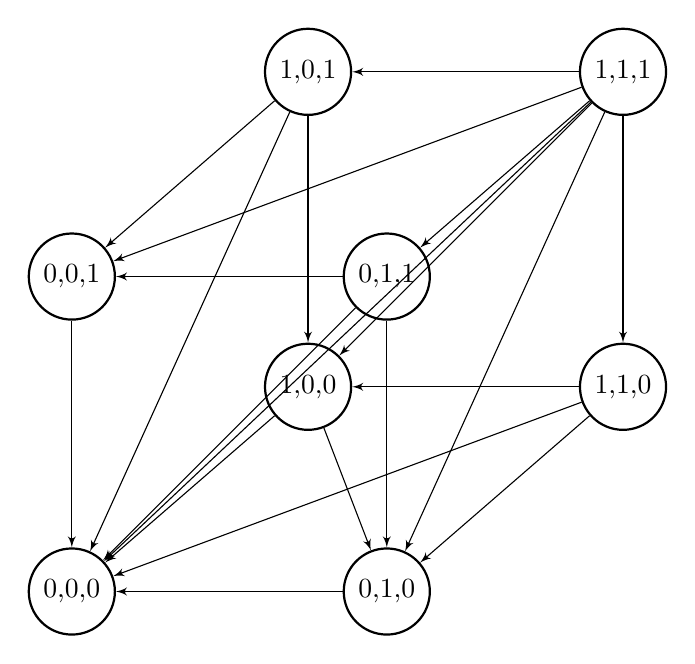
\begin{tikzpicture}
\begin{scope}[every node/.style={circle,thick,draw}]
\node (0) at (0, 0) {0,0,0};
\node (1) at (0, 4) {0,0,1};
\node (2) at (4, 0) {0,1,0};
\node (3) at (4, 4) {0,1,1};
\node (4) at (3, 2.6) {1,0,0};
\node (5) at (3, 6.6) {1,0,1};
\node (6) at (7, 2.6) {1,1,0};
\node (7) at (7, 6.6) {1,1,1};

\draw[edge] (1) to (0);
%\draw[edge] (2) to (1);
\draw[edge] (2) to (0);
\draw[edge] (3) to (0);
\draw[edge] (3) to (1);
\draw[edge] (3) to (2);
\draw[edge] (4) to (0);
%\draw[edge] (4) to (1);
\draw[edge] (4) to (2);
%\draw[edge] (4) to (3);
\draw[edge] (5) to (0);
\draw[edge] (5) to (1);
%\draw[edge] (5) to (2);
%\draw[edge] (5) to (3);
\draw[edge] (5) to (4);
\draw[edge] (6) to (0);
%\draw[edge] (6) to (1);
\draw[edge] (6) to (2);
%\draw[edge] (6) to (3);
\draw[edge] (6) to (4);
%\draw[edge] (6) to (5);
\draw[edge] (7) to (0);
\draw[edge] (7) to (1);
\draw[edge] (7) to (2);
\draw[edge] (7) to (3);
\draw[edge] (7) to (4);
\draw[edge] (7) to (5);
\draw[edge] (7) to (6);

\end{scope}
\end{tikzpicture}
\caption{Transitions between (B,C,D) = (8,10,12) substates}
\label{fig:cube}
\end{figure}

\begin{figure}
  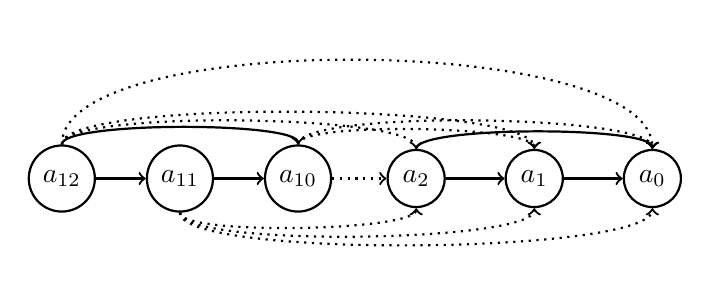
\begin{tikzpicture}[node distance={15mm}, thick, main/.style = {draw, circle}]
\node[main] (6) {$a_{12}$};
\node[main] (5) [right of=6] {$a_{11}$};
\node[main] (4) [right of=5] {$a_{10}$};

\node[main] (3) [right of=4] {$a_{2}$};
\node[main] (2) [right of=3] {$a_1$};
\node[main] (1) [right of=2] {$a_0$};
\draw[->] (6) -- (5);
\draw[->] (6) to [out = 90, in = 90, looseness=.25] (4);
\draw[->] (5) -- (4);

\draw[->] (3) -- (2);
\draw[->] (2) -- (1);
\draw[->] (3) to [out = 90, in = 90, looseness=.25] (1);

\draw[dotted][->] (6) to [out = 90, in = 90, looseness=.25] (3);
\draw[dotted][->] (6) to [out = 90, in = 90, looseness=.25] (2);
\draw[dotted][->] (6) to [out = 90, in = 90, looseness=.5] (1);

\draw[dotted][->] (5) to [out = 270, in = 270, looseness=.25] (3);
\draw[dotted][->] (5) to [out = 270, in = 270, looseness=.25] (2);
\draw[dotted] [->](5) to [out = 270, in = 270, looseness=.25] (1);

\draw[dotted][->](4) -- (3);
\draw[dotted][->](4) to [out = 90, in = 90, looseness=.25] (2);
\draw[dotted][->](4) to [out = 90, in = 90, looseness=.25] (1);

\end{tikzpicture}
\caption{Transitions between 6-die substates}
\label{fig:test2}
\end{figure}





Solving the game perfectly for the standard ``bitches'' setup (15 dice of various sizes) requires evaluating the expected value of 103 different states with a max of 5,940,480 possibilities per state. 

\section{Splitting into parallel games} \label{section:split-out}

We can reduce the game by considering 15 dice as each playing separate one-die games and bear the cost when this ends up being untrue.

\section{Expected Score} \label {section:final-ev} 
The expected score at the end can then be approximated readily.



\end{document}
